\section{Block-based Symmetry Breaking}
\label{sec::blocks2}

The idea we develop in this section 
is to localise straight-move jump points with bitwise operations.  
This implementation allows to manipulate 
many nodes rapidly, 
improving the overall runtime.  

\begin{figure}[ht]
  \begin{center}
    \scalebox{0.8}{%
      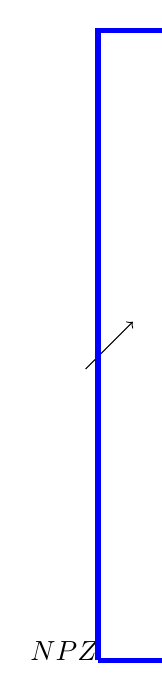
\begin{tikzpicture}
        \creategrid{8}{9}
        \drawobstacle{1}{9}
        \drawobstacle{7}{4}
        \drawobstacle{6}{4}
        \drawobstacle{3}{7}
        \drawobstacle{2}{2}
        \drawobstacle{3}{2}
        \draw[->] (0.7,3.7) -- (1.3,4.3);
        \drawgridnode{2}{5}{$N$}
        \drawgridnode{1}{4}{$P$}
        \drawgridnode{7}{5}{$Z$}
        \drawgridnode{2}{6}{{\color{red} 1}}
        \drawgridnode{1}{5}{{\color{red} 2}}
        \drawgridnode{3}{5}{{\color{red} 3}}
        \drawgridnode{2}{7}{{\color{red} 4}}
        \drawgridnode{1}{6}{{\color{red} 5}}
        \drawgridnode{3}{6}{{\color{red} 6}}
        \drawgridnode{2}{8}{{\color{red} 7}}
        \drawgridnode{1}{7}{{\color{red} 8}}
        \drawgridnode{3}{7}{{\color{red} \bf 9}}
        \draw[blue,line width=2pt] (0,0) -- (0,8) -- (1,8) -- (1,0) -- (0,0);
      \end{tikzpicture}%
    }
  \end{center}
  \caption{A current search state 
    (the grid is assumed larger than the part presented).
  The red numbers show in which order the traversability of the nodes 
  is tested.}
  \label{fig::gridforblocks}
\end{figure}

Consider the grid presented on Figure~\ref{fig::gridforblocks} 
(this is supposed to be a small chunk of a larger grid).  
The node currently being explored is $N$ ($\langle 2,5\rangle$)
and its parent is $P$.  
At this stage, the horizontal and vertical axes must be scanned 
for jump point before a diagonal move to $\langle 3,6\rangle$ is taken.  
As it turns out, two jump points will be found in $4$ and $Z$.  
When looking for a jump point on column $2$, 
the status (traversable or not) of the nodes 
will be checked in the order given by the numbers in red.  
Each one of these nodes will be individually tested.  

However, because of the way the map is stored, 
i.e., each node is represented by a single bit, 
it is possible to manipulate large blocks of data.  
The status of the eight nodes in the blue rectangle in the figure 
could for instance be represented by a single byte $B$ 
whereby the $i$th bit $B[i]$ of the byte is set to $1$ 
iff the node $\langle 0,i\rangle$ of the grid contains an obstacle.  
(Practically, we use 32-bit words 
to represent 32-long rectangles 
but, for simplicity, the discussion will remain on byte.), 
This rectangle in particular contains no obstacle 
and therefore contains no straight-move jump point: 
this can be easily found by noting that $B = 0$.  

More generally, even if the node contains obstacles, 
the jump points can easily be spotted.  
Looking at column $3$, a (potential) jump point 
is defined by an obstacle ($\langle 3, 7\rangle$) 
followed by an empty square ($\langle 3,8\rangle$).  
It is only a potential jump point 
because an obstacle on the current column (here $2$) 
could block the path to the jump point.  

Given a byte $B$ from current row $k$, the potential jump points 
can be found by calculating \texttt{(!(B>>k)\&(B>>1+k))<<k}.  
Any $1$ in the resulting byte is a potential jump point.  
It is possible to extract the position of the first jump point 
using the C command WHAT COMMAND SHOULD BE USED HERE?

For both columns around the current column, 
we compute the first potential jump point (if any): 
we called them $p_1$ and $p_2$.  
In the example of the figure, $p_1$ is undefined 
(in practice, $p_1 > 0$) and $p_2 = 8$.  
Furthermore, we compute the position 
of the first obstacle on the current column, 
to decide whether the first potential jump point is reachable.  
This is done by computing \texttt{(B>>k<<k)} 
and extracting the first bit that evaluates to $0$.  
This value is written $p$.  

Given the three values $p$, $p_1$, and $p_2$, 
three decisions may be taken: 
\begin{itemize}
\item 
  None of them is defined: 
  there is no obstacle on the current row 
  and no potential jump point on the side.  
  We jump to row $8$ and continue with the next rectangle. 
\item 
  Variable $p$ is defined and either the $p_i$s are undefined 
  or their value is bigger than or equal to $p$: 
  the search stops as an obstacle is met.  
\item 
  At least one variable $p_i$ is defined, 
  it is lower than the other two variables (if defined): 
  the first potential jump point is reachable.  
  We jump to row $p_i-1$.  
\end{itemize}
Practically, undefined value are represented by values 
bigger than the size of the word.  
Notice also that, because we consider 32-bit words 
rather than $8$-bit bytes, 
the number of nodes processed in one go 
is much more important than may appear.  
The $64$-bit implementation is more tricky 
as C does not seems to implement natively 
THE COMMANDS TO ACCESS THE BITS SET TO 1.  

\paragraph{Remarks}: 
Whether the last node of the rectangle is a jump point 
cannot be decided.  
The rectangle therefore overlap.  
For instance, if a first rectangle stretches 
from $\langle 2,1\rangle$ to $\langle 2,8\rangle$, 
then the second rectangle will stretch 
from $\langle 2,8\rangle$ to $\langle 2,15\rangle$.  

There is additional redundancy in the map: 
two copies of the map are provided, 
one to search for vertical jump points 
and the other one to search for horizontal jump points.  

%EOF 
